% Software License Agreement
%
% Author    Mike Purvis <mpurvis@clearpathrobotics.com>
% Copyright (c) 2014, Clearpath Robotics, Inc., All rights reserved.
%
% Redistribution and use in source and binary forms, with or without modification, is
% not permitted without the express permission of Clearpath Robotics.

\documentclass[]{clearpath-latex/clearpath-manual}
\graphicspath{{gen/}}
\usepackage{float}
\usepackage{fancyhdr}
\pagestyle{fancyplain}
\lfoot{Rev. 1.1.5}
\rfoot{Jackal UGV}
\lhead{}         
\chead{}              
\rhead{}  
\renewcommand{\headrulewidth}{0pt}





\begin{document}

\manualcover{cover-page.pdf}
\tableofcontents

\section{Introduction}

Jackal is a rugged, lightweight, fast, and easy-to-use unmanned ground vehicle for ROS
Indigo, presented by Clearpath Robotics.

Jackal includes a standard internal PC, as well as basic IMU. Standard
perception modules are available, including URDF and simulator integration, and
demonstration applications.

Please inquire with Clearpath Robotics for details. See \nameref{contact} on page
\pageref{contact} for contact information.

\subsection{What's Included}

Contained in your Jackal shipment are the following items:

\begin{itemize}[nolistsep]
  \item Jackal UGV
  \item 270 watt-hour lithium battery pack
  \item 110V/220V universal charger
  \item Sony Bluetooth controller
  \item Jackal User Manual
\end{itemize}

If you elected to purchase standard payload modules or custom integration services with
Jackal, then additional equipment will be included per your specific configuration, plus
further documentation as required.

\subsection{Hardware Overview}

Jackal's external features include the mounting pattern on the lid panel, \SI{190}{\mm} diameter
wheels, human machine interface panel (HMI), and lid panel latches. The HMI panel is shown in
\autoref{hmi}, and includes from left: motor button, comms indictor, wifi indicator, battery
indicator, and system power button.

% TODO: Labeled drawing of external features.

\begin{figure}[ht]
  \centering
  \includegraphics[width=8.0cm]{hmi.pdf}
  \caption{HMI panel.}
  \label{hmi}
\end{figure}


\begin{figure}[pt]
  \centering
  \def\svgwidth{12cm}
  \input{gen/battery-view.pdf_tex}
  \caption{Battery area inside Jackal.}
  \label{int}
\end{figure}

\begin{figure}[pb]
  \centering
  \def\svgwidth{14cm}
  \input{gen/user-tray.pdf_tex}
  \caption{Computer and user tray.}
  \label{tray}
\end{figure}

To access Jackal's interior, actuate the latches under the front end of the lid, on the opposite end from
the HMI. When you lift the lid, you will see Jackal's onboard Li-Ion battery pack, and its two connectors.
The large Anderson Power Pole connector is to supply power to Jackal and must be connected in order for
Jackal to operate. The smaller white Molex connector allows the battery pack to be charged inside Jackal 
while Jackal is powered off. It is recommended to connect both. The interior components of Jackal are
labeled in \autoref{int}.

Finally, you may undo the thumbscrews which hold Jackal's computer tray to the lid. The tray lowers,
revealing Jackal's onboard Mini-ITX PC, user power supplies, and internal user hardware mounting area.
Please see \autoref{tray} and \autoref{upb} for the components of the tray and user power supplies.
Note that the fused user power is available as four-pin Molex connectors, or a plug-in screw terminal
block. For more information on integrating payloads electrically, see \autoref{payload-elec},
\nameref{payload-elec}.

\begin{figure}[hb]
  \centering
  \def\svgwidth{15cm}
  \input{gen/user-power.pdf_tex}
  \caption{User power supply.}
  \label{upb}
\end{figure}

\subsection{System Architecture}

Like many ROS robots, Jackal is built around an x86 PC running Ubuntu, paired with a
32-bit MCU. The MCU handles IO, power supply monitoring, and motor control, as well as
supplying data from the integrated IMU and GPS receiver. The communication channel
between the MCU and PC is a Full Speed USB connection, with the MCU operating as a
standard serial CDC device.

The communication protocol used is rosserial. An instance of the \lstinline{rosserial_server}
serial node is embedded in the \lstinline{jackal_base} node, where it is connected to
Jackal's kinematic controller.

The key topics which comprise Jackal's ROS API are given in \autoref{table:rosapi}.

% TODO: Data flow diagram
\bgroup
\begin{table}[htp]
\begin{tabular}{  l  l  p{7cm} }
\hline
Topic & Message Type & Purpose \\ \hline

\lstinline!/cmd_vel! & \lstinline!geometry_msgs/Twist! & 
Input to Jackal's kinematic controller. Publish here to make Jackal go. \\ \hline
\lstinline!/odometry/filtered! & \lstinline!nav_msgs/Odometry! & 
Published by \lstinline!robot_localization!, a filtered localization estimate based
on wheel odometry (encoders), and integrated IMU. \\ \hline

\lstinline!/imu/data! & \lstinline!sensor_msgs/IMU! & 
Published by \lstinline!imu_filter_madgwick!, an orientation estimate based on Jackal's
internal gyroscope, accelerometer, and magnetometer. \\ \hline
\lstinline!/navsat/fix! & \lstinline!sensor_msgs/NavSatFix! & 
Position fix from Jackal's built in GPS receiver. \\ \hline
\lstinline!/navsat/vel! & \lstinline!geometry_msgs/TwistStamped! & 
Velocity over ground according to the integrated GPS receiver.\\ \hline

\lstinline!/cmd_drive! & \lstinline!jackal_msgs/Drive! &
Output from Jackal's kinematic controller, input to the motor controllers. Subscribe here for a lower-level look at what's going on. \\ \hline
\lstinline!/feedback! & \lstinline!jackal_msgs/Feedback! &
High-frequency inputs from Jackal's encoders and motor current sensors. \\ \hline
\lstinline!/status! & \lstinline!jackal_msgs/Status! &
Low-frequency status data for Jackal's systems. This information is republished in human
readable form on the \lstinline!diagnostics! topic and is best consumed with the Robot
Monitor. \\ \hline
\end{tabular}
\caption{Jackal ROS API Topics}
\label{table:rosapi}
\end{table}
\egroup


% TODO: Consider moving this content to ROS wiki?


\begin{comment}
\autoref{arch} is a high-level overview of the ROS
nodes in base Jackal and the data flow through them.

\begin{figure}[hb]
  \centering\footnotesize
  \placeholder{16cm}{18cm}
  \caption{ROS nodes and topics on Jackal.}
  \label{arch}
\end{figure}
\end{comment}

\section{Getting Started}

The first step is to power up your Jackal and have some fun driving it around! If you've
just unpacked Jackal from its shipment packaging, you'll need to open it up and connect the
battery.

Press the power button \raisebox{-0.4em}{\includegraphics[width=0.5cm]{icon-power.pdf}} on
Jackal's HMI panel. The LEDs should show a test pattern, after which you will wait about 30
seconds for the internal PC to finish booting up.

% TODO: Add this content back when the comms LED actually works.
% When the comms LED (\raisebox{-0.4em}{\includegraphics[width=0.5cm]{icon-comms.pdf}}) is
% green, this signals that the PC is finished booting up, and that the PC and MCU are in
% communication. At this point, 
  
Press the PS/P3 button on the Sony Bluetooth controller to sync the controller to Jackal. Once
the small red LED on the controller goes solid, you're paired and ready to drive. Hold the L2 trigger
button, and push the thumbstick forward. For full speed mode, switch to the L1 trigger.

If you're not seeing any action, check \nameref{trouble} on page \pageref{trouble} to
get in touch with support.

\subsection{Wireless Access}

To get Jackal connected to your local wifi, you must first access the internal computer
using a wired connection. Open the chassis, lower the computer tray, and connect to the network port
labeled \lstinline{STATIC} with a standard ethernet cable. 

\subsubsection{Static IP Configuration}

Set your laptop's ethernet port to a static IP such as \lstinline{192.168.1.51}.  To do this in Ubuntu, follow the steps below: 
\begin{enumerate}
  \item Click on the Wifi icon in the upper-right corner of your screen, and select \textbf{Edit Connections}
  \item In the \textbf{Network Connections} window, under \textbf{Ethernet}, select your wired connection and then click \textbf{Edit}
  \item Select the \textbf{IPv4 Settings} tab and then change the \textbf{Method} to \lstinline{Manual}
  \item Click the \textbf{Add} button to add a new address
  \item Enter a \lstinline{192.168.1.51} as the static IP under the \textbf{Address} column, and enter \lstinline{255.255.255.0} under the \textbf{NetMask} column, and then select \textbf{Save}
\end{enumerate}

\begin{figure}[H]
  \centering
  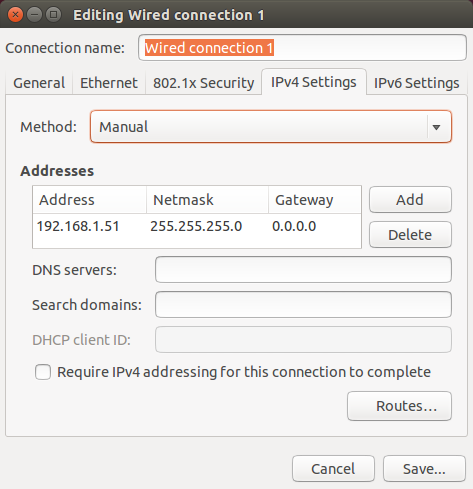
\includegraphics[width=0.5\linewidth]{wired_connection.PNG}
  \caption{Static IP Configuration}
  \label{staticip}
\end{figure}
            

\subsubsection{Connect to Jackal via SSH over ethernet}

The next step is to connect to Jackal via SSH.  To do so execute the following in a terminal window:

\begin{lstlisting}
ssh administrator@192.168.1.11
\end{lstlisting}

You will be promoted to enter a password.  The default password is \lstinline{clearpath}.

\subsubsection{Connect Jackal to Wireless Network}

Now that you're connected via SSH over a wired connection, you can setup Jackal to connect to a local wifi network.  To do this, you will use the wireless interface configuration daemon (WICD) - a preinstalled network manager.  

In a terminal window, execute the following command:

\begin{lstlisting}
wicd-curses
\end{lstlisting}

You should see a browsable list of networks which the robot has detected. Use arrow keys to select the one you would like to connect to, and then press the right arrow to configure it. You can enter your network’s password near the bottom of the page, and note that you must select the correct encryption scheme; most modern networks use WPA1/2 Passphrase, so if that’s you, make sure that option is selected. You also likely want to select the option to automatically reconnect to this network, so that Jackal will be there for you on your wireless automatically in the future.  

When you’re finished, press \textbf{F10} to save, and then \textbf{C} to connect.  Jackal is now connected to wifi!  

While you're still wired to Jackal, you'll need to identify the IP address of Jackal's wireless connection.  

In a terminal window, execute:

\begin{lstlisting}
ifconfig
\end{lstlisting}

A list of network connections will be displayed within the terminal.  Locate the wireless network and make note of its IP address. Now that you know Jackal's wireless IP address, you may now exit the ethernet SSH session by executing \lstinline{exit}.

Remove the ethernet cord and close up Jackal.   Now you can SSH into Jackal over the wireless network.  To do so, execute:

\begin{lstlisting}
ssh administrator@<IP_OF_JACKAL>
\end{lstlisting}

SSH sessions allow you to control Jackal's internal computer.  You can do various things such as download packages, run updates, add/remove files, transfer files etc. 

\subsection{Remote ROS Connectivity}\label{remote}

To use ROS desktop tools, you’ll need your computer to be able to connect to Jackal’s ROS master. This will allow you to run ROS commands like \lstinline{rostopic list}, \lstinline{rostopic echo}, \lstinline{rosnode list}, and others, from a remote PC and the output will reflect the activity on Jackal’s ROS master, rather than on your own machine.  This can be a tricky process, but we’ve tried to make it as simple as possible.

In order for the ROS tools on your computer to talk to Jackal, they need to know two things:

\begin{itemize}[nolistsep]
  \item How to find the ROS master, which is set in the \lstinline{ROS_MASTER_URI} environment variable, and
  \item How processes on the other computer can find your computer, which is the \lstinline{ROS_IP} environment variable.
\end{itemize}

The suggested pattern is to create a file in your home directory called \lstinline{remote-jackal.sh} with the following contents:

\begin{lstlisting}
export ROS_MASTER_URI=http://cpr-jackal-0001:11311  # Jackal's hostname
export ROS_IP=10.25.0.102       # Your laptop's wireless IP address
\end{lstlisting}

If your network doesn’t already resolve Jackal’s hostname to its wireless IP address, you may need to add a corresponding line to your computer’s /etc/hosts file:

\begin{lstlisting}
10.25.0.101 cpr-jackal-0001
\end{lstlisting}

\textbf{NOTE:} You can verify the hostname and IP address of Jackal using the following commands during an SSH session with the onboard PC.

\begin{lstlisting}
hostname
hostname -i
\end{lstlisting}

Then, when you’re ready to communicate remotely with Jackal, you can source that script like so, thus defining those two key environment variables in the present context.

\begin{lstlisting}
source remote-jackal.sh
\end{lstlisting}

To verify that everything is set up propelry, try running a few ROS commands, such as the standard visual ROS tools:

\begin{lstlisting}
roslaunch jackal_viz view_robot.launch
rosrun rqt_robot_monitor rqt_robot_monitor
rosrun rqt_console rqt_console
\end{lstlisting}

If the tools launch, then everything is setup properly. 

Please contact Clearpath Support if you need assistance in conifugring remote access. For more general details on how ROS works over TCP with multiple machines, please see:

\url{http://wiki.ros.org/ROS/Tutorials/MultipleMachines}.

For help troubleshooting a multiple machines connectivity issue, see:

\url{http://wiki.ros.org/ROS/NetworkSetup}

\newpage\subsection{Jackal Desktop Packages}

To command or observe Jackal from your desktop computer, first set up a basic
ROS installation. See the following page for details:

\url{http://wiki.ros.org/indigo/Installation/Ubuntu}

When your ROS install is set up, install the Jackal desktop packages:

\begin{lstlisting}
sudo apt-get install ros-indigo-jackal-desktop
\end{lstlisting}

Once your remote access to Jackal's ROS master is configured (see options in \autoref{remote}),
you can launch rviz, the standard ROS robot visualization tool:

\begin{lstlisting}
roslaunch jackal_viz view_robot.launch
\end{lstlisting}

From within rviz, you can use interactive markers to drive Jackal, you can visualize its
published localization estimate, and you can visualize any attached sensors which have been
added to its robot description XML (\lstinline{URDF}).

Additionally from the desktop, you can launch the standard RQT Robot Monitor, which
watches the diagnostic output from Jackal's self-montoring capabilities:

\begin{lstlisting}
rosrun rqt_robot_monitor rqt_robot_monitor
\end{lstlisting}

% TODO: Insert images of robot monitor/GUI and rviz window.

% TODO: Add "finishing up" section about turning Jackal off and connecting the charger.

\section{Apps}

When equipped with a laser scanner as is available in the Gazebo simulation, Jackal works with the
standard ROS navigation stack. See \url{http://wiki.ros.org/jackal_navigation}.

A standard outdoor GPS autonomy demonstration using Jackal's built-in sensing is planned, as well
as a calibration app for the internal magnetometer.


\section{Charging \& Battery Maintenance}

Jackal's Li-Ion battery pack may be charged internal to the chassis---simply plug in
the charger to the charge port located under the rear fender. Charging will occur
when Jackal is powered down.

Alternatively, if you have multiple battery packs, you can easily lift the lid and
remove the battery for external charging. When charging externally, remove the pigtail
which adapts the charger to the platform's weather sealed charge port.

The battery pack is manufactured for Clearpath Robotics by AllCell Technologies. The
pack includes integrated protections against fault due to overcurrent, overdischarge,
and short circuit. The pack is rugged and designed for the demanding environments into
which Jackal may be deployed.

However, please take note of the following:

\begin{itemize}
\item The pack must not be stored or operated above \SI{60}{\celsius} or below \SI{-19}{\celsius}.
\item The pack must not be punctured or disassembled.
\item The pack should be dropped off or delivered to your local hazardous waste authority for disposal.
\item When traveling with Jackal, consult your airline's restrictions regarding lithium
battery packs. If possible, bring the pack in your carry on luggage, where it will
be subject to normal cabin temperatures and pressures.
\end{itemize}

Please contact Clearpath Robotics for additional information about Jackal's battery or
for information about purchasing additional packs.


\section{Payload Integration Guide}

If you're wanting to attach custom hardware to Jackal, you'll have to take care of
mechanical mounting, electrical supply, and software integration. This section
aims to equip you with respect to these challenges.

% TODO: Images throughout this section.

\subsection{Mechanical Mounting}

For external payloads, the recommended configuration is manufacture a metal or plastic bracket
which attaches to the \SI{120}{\mm} square mounting holes supplied in Jackal's lid
panel. The included thumbscrews use an M5 thread, if you wish to replace them with conventional
fasteners. As an alternative to manufacturing a brand new plate, you may remove and modify one
of the included ones.

For rear-facing or back-mounted payloads, it is also possible to replace (or drill into) the
hatch panel which covers over access to Jackal's internal PC.

\subsection{Electrical Integration}\label{payload-elec}

Except for bus-powered USB cameras, most payloads have separate leads for power and data. Data
connections may be brought through the hatch and connected directly to the internal computer. Both
of Jackal's internal computer options support USB3 and Ethernet connectivity. With the performance
PC, the PCIe slot may be used to supply Firewire, Thunderbolt, or additional USB3 ports, as necessary.

Additionally, the internal mounting area may be used for an Ethernet switch, when attaching multiple
Ethernet payloads, or for a PoE power injector as required.

The power lead may likewise be brought through the hatch, and connected to the User Power Board. Pull
out the black terminal block, and use a small screwdriver to securely attach power leads to it.
Confirm voltage and polarity before reconnecting the terminal block.

You may also choose to terminate your payload's power lead with the appropriate crimps and pins
for the four pin Molex connector--- this option may be more convenient if you expect to be adding
and removing your payload from Jackal more frequently and would prefer not to be fiddling with the
terminal block. The Digi-key part number for the matting connector is WM3701-ND and the pins used are WM2501CT-ND.


\subsection{Software Integration}

ROS has a large ecosystem of sensor drivers, some of which include pre-made URDF descriptions and
even simulation configurations. Please see the following page on the ROS wiki for a partial list:

\url{http://wiki.ros.org/Sensors}

For the best experience, consider purchasing supported accessories from Clearpath Robotics for your
Jackal, which will include simulation, visualization, and driver support. However, we will happily
assist you in integrating your own devices as well.


\section{Contact}\label{trouble}\label{contact}

Clearpath is committed to your success with Jackal. Please get in touch with us and we'll
do our best to get you rolling again quickly: \href{mailto:support@clearpathrobotics.com}{support@clearpathrobotics.com}

To get in touch with a salesperson regarding Jackal or other Clearpath Robotics products, please
email \href{mailto:sales@clearpathrobotics.com}{sales@clearpathrobotics.com}.

If you have a an issue that is specifically about ROS and is something which may be of interest
to the broader community, consider asking it on \href{http://answers.ros.org}{answers.ros.org}.
If you don't get a satisfactory response, please ping us and include a link to your question
as posted there. If appropriate, we'll answer in the ROS Answers context for the benefit of the
community.

Jackal is designed not to require regular maintenance. As it is a newer product, Clearpath
appreciates your patience as we understand its weak-point components and fill out the appropriate
care instructions for the platform.

\end{document}
